% !TeX encoding=utf-8
\documentclass[a4paper]{feidippp}
\usepackage[pdftex]{graphicx}
\DeclareGraphicsExtensions{.pdf,.png.,mps.,jpg}
\graphicspath{{figures/}}

\usepackage[utf8]{inputenc}
\usepackage[T1]{fontenc}
\usepackage{listings}
\usepackage{color}

\definecolor{codegreen}{rgb}{0,0.6,0}
\definecolor{codegray}{rgb}{0.5,0.5,0.5}
\definecolor{codepurple}{rgb}{0.58,0,0.82}
\definecolor{backcolour}{rgb}{0.95,0.95,0.92}

\lstdefinestyle{mystyle}{
    backgroundcolor=\color{backcolour},   
    commentstyle=\color{codegreen},
    keywordstyle=\color{magenta},
    numberstyle=\tiny\color{codegray},
    stringstyle=\color{codepurple},
    basicstyle=\footnotesize,
    breakatwhitespace=false,         
    breaklines=true,                 
    captionpos=b,                    
    keepspaces=true,                 
    numbers=left,                    
    numbersep=5pt,                  
    showspaces=false,                
    showstringspaces=false,
    showtabs=false,                  
    tabsize=2
}

\lstset{style=mystyle}


\usepackage[slovak]{babel}



\usepackage{lmodern}

\usepackage[document]{ragged2e}

\usepackage{amsmath,amssymb,amsfonts}

\usepackage{listings}

\def\figurename{Obrázok}
\def\tabname{Tabuľka}
 


%\usepackage[dvips]{graphicx}
%\DeclareGraphicsExtensions{.eps}

\usepackage[edges]{forest}

\definecolor{foldercolor}{RGB}{124,166,198}

\tikzset{pics/folder/.style={code={%
    \node[inner sep=0pt, minimum size=#1](-foldericon){};
    \node[folder style, inner sep=0pt, minimum width=0.3*#1, minimum height=0.6*#1, above right, xshift=0.05*#1] at (-foldericon.west){};
    \node[folder style, inner sep=0pt, minimum size=#1] at (-foldericon.center){};}
    },
    pics/folder/.default={20pt},
    folder style/.style={draw=foldercolor!80!black,top color=foldercolor!40,bottom color=foldercolor}
}

\forestset{is file/.style={edge path'/.expanded={%
        ([xshift=\forestregister{folder indent}]!u.parent anchor) |- (.child anchor)},
        inner sep=1pt},
    this folder size/.style={edge path'/.expanded={%
        ([xshift=\forestregister{folder indent}]!u.parent anchor) |- (.child anchor) pic[solid]{folder=#1}}, inner xsep=0.6*#1},
    folder tree indent/.style={before computing xy={l=#1}},
    folder icons/.style={folder, this folder size=#1, folder tree indent=3*#1},
    folder icons/.default={12pt},
}

%\usepackage[pdftex]{hyperref} %% tlac !!!
\usepackage[pdftex,colorlinks,citecolor=magenta,bookmarksnumbered,unicode,pdftoolbar=true,pdfmenubar=true,pdfwindowui=true,bookmarksopen=true]{hyperref}
\hypersetup{%
baseurl={http://www.tuke.sk/sevcovic},
pdfcreator={pdfcsLaTeX},
pdfkeywords={Používateľská priručka},
pdftitle={Simulácia kooperácie multi-robotickéhosystému},
pdfauthor={Bohdan Tanasov},
pdfsubject={Používateľská priručka}
}

% Citovanie podla mena autora a roku
%\usepackage[numbers]{natbib}
\usepackage{natbib} \citestyle{chicago}

%\usepackage{mathptm} %\usepackage{times}

\katedra{umelej inteligencie}
\department{Fakulta elektrotechniky a informatiky}
\odbor{Inteligentné systémy}
\autor{Bohdan Tanasov}
\veduci{doc. Dr. Ing.~Ján~Vaščák}
\konzultant{doc. Dr. Ing.~Ján~Vaščák}
\nazov{Simulácia kooperácie multi-robotického systému}
% \kratkynazov{Optimalizácia písania DP}
\nazovprogramu{Proces multi-robotického lovu}
\klucoveslova{optimalizácia, diplomová práca, písanie}
\title{The optimization of the diploma writing at our faculty}
\keywords{optimization, diploma, writing}
\datum{28. 5. 2021}



\begin{document}
\bibliographystyle{dcu}



\titulnastrana

\newpage


\tableofcontents

\newpage

\addcontentsline{toc}{section}{\numberline{}Zoznam obrázkov}
\listoffigures

\newpage


\setcounter{page}{1}

\section{Funkcia programu}

Tento program je súčasťou bakalárskej práce a týka sa experimentov s kooperatívnymi úlohami vykonávaných rôznymi typmi
 robotov. Toto riešenie obsahuje projekt, ktorý simuluje proces lovu so skupinou multi-robotov pripravených v ROS2 a 
 simulovaných v prostredí Webots. Simulácia je plocha s modelmi rôznych fyzických objektov, robotov a algoritmov na ich riadenie.

\vspace{3mm}

\justifying
\noindent
Používateľ má možnosť sledovať experiment v reálnom čase pomocou grafického okna a ovládať simulačný čas pomocou ovládacích tlačidiel a klávesnice. Webots umožňujú vytvoriť zo simulácie applet alebo video HTML.

\section{Inštalácia programu}

\subsection{Požiadavky na technické prostriedky}
Na spustenie projektu je potrebný nasledujúci hardvér:
\begin{itemize}
    \item Pomerne nedávny počítač typu PC alebo Mac s minimálne dvojjadrovým taktom procesora 2 GHz a 2 GB pamäte RAM je minimálnou požiadavkou. Odporúča sa však štvorjadrový procesor. Minimalne 4 GB diskoveho priestoru.
    \item Vyžaduje sa grafický adaptér s podporou NVIDIA alebo AMD OpenGL (minimálna verzia 3.3) s minimálne 512 MB RAM. Neodporúča sa žiadne ďalšie grafické adaptéry, vrátane grafických adaptérov Intel, pretože im často chýba dobrá podpora OpenGL, čo by mohlo spôsobiť problémy s 3D vykresľovaním a zlyhania aplikácií. Napriek tomu v niektorých prípadoch môže inštalácia najnovšieho grafického ovládača Intel tieto problémy vyriešiť a umožniť vám používať Webots. Na toto však neposkytujeme žiadnu záruku. Pre systémy Linux odporúčam iba grafické karty NVIDIA. Project funguje dobre na všetkých grafických kartách obsiahnutých v pomerne nedávnych počítačoch Apple.
\end{itemize}

\subsection{Požiadavky na programové prostriedky}
% Toto riešenie je vytvorené pomocou nasledujúcich verzií softvéru:
\begin{enumerate}
\item Webots – R2020a revision 1. Toto riešenie bolo vyvinuté a spustené na verzii We-bots: R2020a revízia 1. Webots je možné prevádzkovať na systémoch Ubuntu Linux LTS 18.04, Windows 8.1 alebo Windows 10 a Mac OS 10.15 „Catalina“ a 10.14 „Mojave“.
\item Python – 3.6.9. Toto riešenie obsahuje programy (radiče) Pythonu, takže sa vyžaduje aj prostredie Pythonu.
\item Pip – 9.0.1. Toto je správca balíkov Python na inštaláciu ďalších knižníc.
\item NumPy – 1.18.4. Je to knižnica Pythonu pre matematické operácie a v tomto riešení sa používajú niektoré funkcie.
% \item Linux - Ubuntu 20.04
% \item Visual Studio code
\item ROS - 2. ROS, robotický operačný systém, je platformou voľby pre vývoj robotov.
\item OpenCV – 4.5.2. OpenCV poskytuje knižnicu, nástroje a hardvér počítačového videnia optimalizovanú v reálnom čase.
\end{enumerate}

\subsection{Vlastná inštalácia}

Táto časť obsahuje proces inštalácie systému Ubuntu Linux (18.04) pomocou nástroja Advanced Package Tool. Prosím, otvorte terminál a postupne spustite nasledujúce príkazy na inštaláciu Webots:

\begin{lstlisting}[language=Python, caption=Python example]
$ wget -qO- https://cyberbotics.com/Cyberbotics.asc 
    | sudo apt-key add -

$ sudo apt-add-repository 
    "deb https://cyberbotics.com/debian/ binary-amd64/"

$ sudo apt-get update

$ sudo apt-get install webots
\end{lstlisting}
\vspace{3mm}

\justifying
\noindent
Potom spustite nasledujúce príkazy na inštaláciu Pythonu a požadovaných knižníc:

\begin{lstlisting}
$ sudo apt-get update

$ sudo apt install software-properties-common

$ sudo add-apt-repository ppa:deadsnakes/ppa

$ sudo apt-get update

$ sudo apt-get install python3

$ sudo apt-get install pip3

$ pip install numpy

$ pip install opencv-python

\end{lstlisting}
\vspace{3mm}

\justifying
\noindent
Ďalším krokom je inštalácia ROS2.
\vspace{3mm}

\justifying
\noindent
Krok 1. Set locale
\begin{lstlisting}
$ locale  # check for UTF-8

$ sudo apt update && sudo apt install locales
$ sudo locale-gen en_US en_US.UTF-8
$ sudo update-locale LC_ALL=en_US.UTF-8 LANG=en_US.UTF-8
$ export LANG=en_US.UTF-8
    
$ locale  # verify settings
\end{lstlisting}
\vspace{3mm}

\justifying
\noindent
Krok 2. Add the ROS 2 apt repository
\begin{lstlisting}
$ sudo apt update && sudo apt install curl gnupg2 lsb-release

$ sudo curl -sSL https://raw.githubusercontent.com/ros/rosdistro
    /master/ros.key  -o /usr/share/keyrings/ros-archive-keyring.gpg

$ echo "deb [arch=$(dpkg --print-architecture) 
    signed-by=/usr/share/keyrings/ros-archive-keyring.gpg] 
    http://packages.ros.org/ros2/ubuntu $(lsb_release -cs) main" | 
    sudo tee /etc/apt/sources.list.d/ros2.list > /dev/null
\end{lstlisting}
\vspace{3mm}

\justifying
\noindent
Krok 3. Install development tools and ROS tools
\begin{lstlisting}
$ sudo apt update && sudo apt install -y \
  build-essential \
  cmake \
  git \
  libbullet-dev \
  python3-colcon-common-extensions \
  python3-flake8 \
  python3-pip \
  python3-pytest-cov \
  python3-rosdep \
  python3-setuptools \
  python3-vcstool \
  wget

$ python3 -m pip install -U \
  argcomplete \
  flake8-blind-except \
  flake8-builtins \
  flake8-class-newline \
  flake8-comprehensions \
  flake8-deprecated \
  flake8-docstrings \
  flake8-import-order \
  flake8-quotes \
  pytest-repeat \
  pytest-rerunfailures \
  pytest

$ sudo apt install --no-install-recommends -y \
  libasio-dev \
  libtinyxml2-dev
  
$ sudo apt install --no-install-recommends -y \
  libcunit1-dev$
\end{lstlisting}
\vspace{3mm}

\justifying
\noindent
Krok 4. Get ROS 2 code
\begin{lstlisting}
$ mkdir -p ~/ros2_foxy/src

$ cd ~/ros2_foxy

$ wget https://raw.githubusercontent.com/ros2/ros2/foxy/ros2.repos

$ vcs import src < ros2.repos
\end{lstlisting}
\vspace{3mm}

\justifying
\noindent
Krok 5. Install dependencies using rosdep and build the code in the workspace
\begin{lstlisting}
$ sudo rosdep init

$ rosdep update

$ rosdep install --from-paths src --ignore-src --rosdistro foxy 
    -y --skip-keys "console_bridge fastcdr fastrtps 
    rti-connext-dds-5.3.1 urdfdom_headers"

$ cd ~/ros2_foxy/

$ colcon build --symlink-install
\end{lstlisting}
\subsection{Popis štruktúry programu}

\begin{forest}
  for tree={font=\sffamily, grow'=1,
  folder indent=.9em, folder icons,
  edge=densely dotted}
  [multihunting
    [launch
          % [ar\char`_detection\char`_launch.py, is file]
          [..., is file]
          ]
    [multihunting
          % [\char`_\char`_init\char`_\char`_.py, is file]
          % [commander.py, is file]
          % [robot\char`_enable.py, is file]
          % [robot\char`_enable\char`_follower.py, is file]
          % % [robot-enable-follower2.py, is file]
          % [robot\char`_enable\char`_lead.py, is file]
          % [teleop\char`_keyboard.py, is file]
          % [teleop\char`_keyboard\char`_listen.py, is file]
          [..., is file]
          ]
    [protos
          % [RobotSense.proto, is file]
          % [RobotSenseCamera.proto, is file]
          % [RobotSenseCameraLead.proto, is file]
          [..., is file]
          ]
    [resource
          % [multihunting, is file]
          [..., is file]
          ]
    [worlds
          [textures
          [..., is file]]
          [..., is file]
          % [custom\char`_ar\char`_tag.wbt, is file]
          ]
      [README.md, is file]
      [package.xml, is file]
      [setup.cfg, is file]
      [setup.py, is file]
  ]
\end{forest}
  \vspace{3mm}

  \justifying
  \noindent
The start point of this simulation is ar-detection-launch.py file located in launch directory. Popis hlavných priečinkov v balíku:

worlds: miesto pre svetove súbory Webots (.wbt), ktorý definuje jedného alebo viacerých robotov a ich prostredie. Súbor .wbt niekedy závisí od externých súborov (.proto), ktore sa nachadza v protos a textúr, ktore v textures;

protos: miesto pre prototypy robotov pre svetový súbor Webots;

multihunting: umiestnene skripty Pythonu, ktoré je možné spustiť priamo a aj so spúšťacím súborom;

launch: miesto pre všetky spúšťacie súbory v balíku;


% \subsection{Popis správ pre systémového programátora}

% Uviest texty správ, ktoré sa vypisujú pocas cinnosti programu, príciny týchto správ, popis programu cinnosti, ktoré je potrebné po týchto správach vykonat.

\section{Použitie programu}
Táto časť obsahuje popis postupu na otvorenie a spustenie simulácie.

\subsection{Running procedure}

Po inštalácii požadovaneHO softvéru môžete spustiť simulaciu. Otvorte terminál v priečinku pracovného priestoru a
spustite nasledujúci príkazi:
\begin{lstlisting}
  $ colcon build
  $ . install/setup.bash
  $ ros2 run multihunting ar-detection-launch.py
\end{lstlisting}

Potom uvidíte, že táto platforma ROS2 spúšťa Webots a simulácia začne. Informácie o simulácii môžete sledovať v termináli.

\subsection{Simmulation control}


Užívateľ môže pomocou panela nástrojov riadiť proces simulácie. Panel s nástrojmi sa nachádza v hornej časti hlavného okna Webots. 
\begin{figure}[ht!]
  \centering
  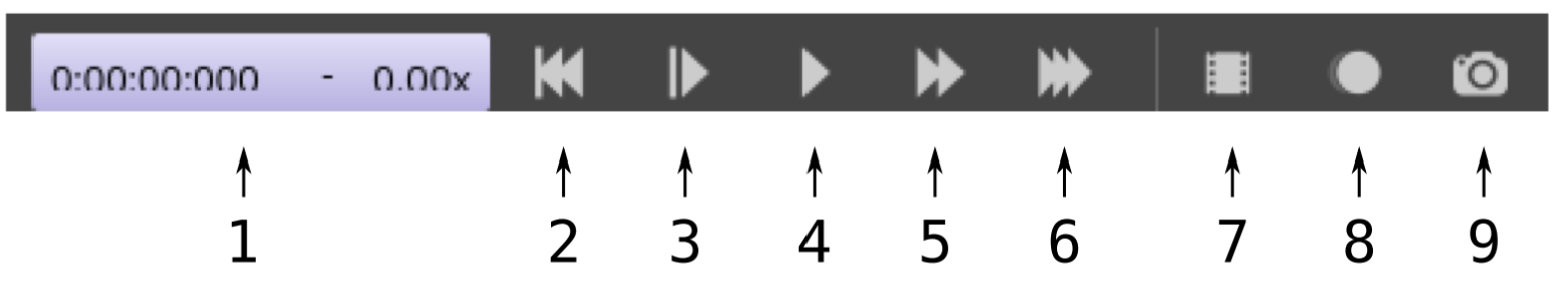
\includegraphics[width=.70\textwidth,angle=0]{1.png}
  \caption{Panel nástrojov Webots.}
  \label{o:1}
\end{figure}
\vspace{3mm}

\justifying
\noindent
Obsahuje nasledujúce prvky(obrazok 3-1.):
\begin{enumerate}
  \item Časová os simulácie a rýchlostná stupnica.
  \item Resetovacie tlačidlo simulácie. Obnoviť počiatočný stav simulácie.
  \item Vykonajte jeden krok.
  \item Spustite simuláciu v reálnom čase.
  \item Spustite simuláciu.
  \item Spustite simuláciu čo najrýchlejšie bez grafiky.
  \item Spustiť videozáznam aktuálnej simulácie.
  \item Spustite záznam animácie HTML5.
  \item Uložte aktuálny obrázok simulácie.
\end{enumerate}

% \textbf{Argumenty ovládačov.} 
% Užívateľ môže pomocou stromu uzlov nastaviť argumenty pre radič.

% \begin{figure}[ht!]
%   \centering
%   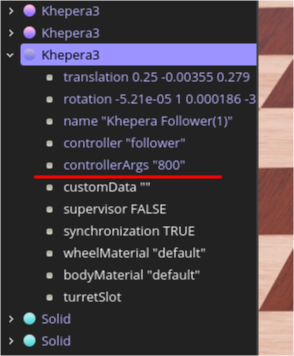
\includegraphics[width=.40\textwidth,angle=0]{2.png}
%   \caption{Strom uzla.}
%   \label{o:2}
% \end{figure}
\subsection{Error Messages}
Môžu sa zobraziť nasledujúce varovania. V prvom prípade jednoducho upozorní na zmenu mierky textúry. Druhý a tretí typ varovaní sa vyskytujú, keď nastane problém s inicializáciou ovládača pre konkrétneho robota. Problém je vyriešený jednoduchým reštartovaním simulácie. Príklad:
\begin{lstlisting}
  WARNING: Texture image size of '/home/bohdan/ros2_ws/install/mybachelorproject/share/mybachelorproject/worlds/textures/loop.jpg' is not a power of two: rescaling it from 1080x1080 to 2048x2048.
  WARNING: Failed to attach extern robot controller: no available "<extern>" robot controller named "follower_Robot_sense" found.
  WARNING: WARNING: Failed to attach extern robot controller: no available "<extern>" robot controller named "follower_Robot_sense" found.
\end{lstlisting}


% \section{Popis vstupných, výstupných a~pracovných súborov} 

% Napr. formáty súborov, atd.

% \section{Obmedzenia programu}

% Zoznam obmedzení programu.

% \section{Chybové hlásenia}

% Chybové hlásenia vlastné pre daný aplikacný program.

% Chybové hlásenia súvisiace s~OS, Štandard. p.~p., \dots).

% \section{Príklad použitia}

% Príklad použitia programu.

% \section{Popis demo-verzie}

% Popis demo-verzie. V~prípade, že navrhovaný program je demo-verzia.


% \addcontentsline{toc}{section}{\numberline{}Zoznam tabuli}
% \listoftables


% \def\refname{Zoznam použitej literatúry}
% \addcontentsline{toc}{section}{\numberline{}Zoznam použitej literatúry}

% \begin{thebibliography}{999}
% \harvarditem{Barančok et al.}{1995}{barancok}
% BARANČOK, D. et al. 1995. \emph{The effect of semiconductor surface treatment on LB film/Si interface.} In:~Physica Status Solidi /a/,  ISSN 0031-8965, 1995, vol. 108, no.2, pp. K~87\,--\,90

% \harvarditem{Gonda}{2001}{gonda}
% GONDA, V. 2001. \emph{Ako napísať a~úspešne obhájiť diplomovú prácu.} Bratislava : Elita, 2001, 3.~doplnené a~prepracované vydanie, 120~s. ISBN 80-8044-075-1

% \harvarditem{Jadr. fyz. a~tech.}{1985}{slovnik}
% \emph{Jadrová fyzika a~technika: Terminologický výkladový slovník.} 2.~rev.~vyd. Bratislava : ALFA, 1985. 235 s. ISBN 80-8256-030-5

% \harvarditem{Katuščák}{1998}{kat}
% KATUŠČÁK, D. \emph{Ako písať vysokoškolské a~kvalifikačné práce.} Bratislava : Stimul, 1998, 2.~doplnené vydanie. 121~s. ISBN 80-85697-82-3

% %\harvarditem{Sýkora a~i.}{1980}{sykora}
% %SÝKORA, F. a~iní. 1980. \emph{Telesná výchova a~šport.} 1.~vyd. Bratislava : SPN, 1980. 35 s. ISBN 80-8046-020-5

% \harvarditem{Lamoš a~Potocký}{1989}{lamos}
% LAMOŠ, F. -- POTOCKÝ, R. 1989. \emph{Pravdepodobnosť a~matematická štatistika.} 1.~vyd. Bratislava : Alfa, 1989. 344 s. ISBN 80-8046-020-5

% %\harvarditem{Sýkora a~i.}{1980}{sykora}
% %SÝKORA, F. a~iní. 1980. \emph{Telesná výchova a~šport.} 1.~vyd. Bratislava : SPN, 1980. 35 s. ISBN 80-8046-020-5

% \harvarditem{Lamoš a~Potocký}{1989}{lamos}
% LAMOŠ, F. -- POTOCKÝ, R. 1989. \emph{Pravdepodobnosť a~matematická štatistika.} 1.~vyd. Bratislava : Alfa, 1989. 344 s. ISBN 80-8046-020-5


% \end{thebibliography}


\end{document}